\section{Array Logic and Notation}\label{sec:arrays}
It is particularly important to understand how arrays are constructed. The rest of the paper relies entirely on the nuances and particularities of this logic and notation. This section is intended for mathematicians and computer scientists. 

\subsection{Logic of the arrays}
The majority of the variables are arrays representing "in order" the different constrained values linked to the solution. The solution to the problem is an array of MIDI notes lists representing counterpoint. Before starting, two constants\footnote{Careful, these are constants from the point of view of the Gecode solver. They are variables defined once with the input but which are never set as constraint variables in the CSP.} must be defined\footnote{These constants are defined more precisely in subsection \ref{sec:constants}.}:

\begin{itemize}
    \item $m$ as the number of measures of the \cf and the counterpoint;
    \item $s_{m}$ as the maximum number of notes possible in the counterpoint, i.e. the size of the main arrays used to store Gecode variables. $s_{m} = m + 3\times (m-1)$ and by extension, $s_{m-1} = (m-1) + 3\times (m-2)$.
\end{itemize}

Intuitively one would separate an array into $m$ lists of each measure with the different notes of a measure inside. Here the reverse applies. With a C-like representation, the access to a variable will be done as $[beat][measure]$ instead of $[measure][beat]$. This is more convenient for applying constraints in Lisp with GiL. Indeed, since the number of beats used by species varies, it is then easier to separate the arrays by lists of beats in order to be able to initialize only those which are treated in the problem. Since these arrays are initialized not with simple integers but with \texttt{IntVar} objects from Gecode, these constraint variables would definitely be initialized in the constraint space, which would not be ideal.\\

All the arrays related directly to the counterpoint are stored in arrays of size $s_{m}$ (or $s_{m-1}$ for the melody arrays as will be explained later). These arrays are composed of four lists, each representing the corresponding beat all along the measures of the song. The first is of size $m$ while the other three are of size $m-1$ since they do not have a note in the last measure of the counterpoint which is only composed of a single whole note. E.g. \texttt{notes[0][9]}\footnote{This array exists only as an example. Here the notation corresponds neither to Lisp notation nor to mathematical notation.} would represent the note in the first beat of the tenth measure.

If the chosen species of counterpoint uses only \textbf{whole notes}, i.e. the first one, each note in first beat of each measure lasts \textbf{four beats}. Consequently, the lists of notes in the second, third and fourth beats are not used because these notes would already be represented by the one in first beat. The same logic applies to the other species: the second and fourth species only use the \textbf{first} and \textbf{third} "beat lists" because a note lasts \textbf{two beats}. While the third and fifth species are the only ones to use the \textbf{four available} beat lists because a note (can) last(s) \textbf{one beat}. See figure \ref{fig:thefourspecies} (the corresponding midi value is annotated below each note) and table \ref{tab:thefourspecies} for clarity.
\begin{figure}[h]
    \centering
    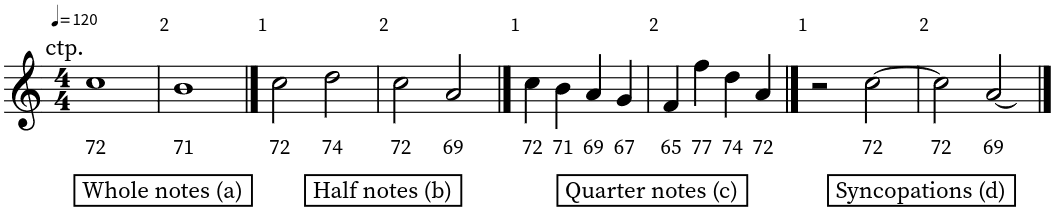
\includegraphics[width=\textwidth]{Images/the_four_species.png}
    \caption{The 3 types of notes (N.B.: b $\equiv$ d) over 8 beats for the \nth{4} first species.}
    \label{fig:thefourspecies}
\end{figure}

\begin{table}[h]
    \centering
    \resizebox{\columnwidth}{!}{%
    \begin{tabular}{|c||c|c|c|c||c|c|c|c|}
        \hline
        beat, measure & \nth{1}, \nth{1} & \nth{2}, \nth{1} & \nth{3}, \nth{1} & \nth{4}, \nth{1} & \nth{1}, \nth{2} & \nth{2}, \nth{2} & \nth{3}, \nth{2} & \nth{4}, \nth{2} \\
        \hline
        \hline
        \hline
        Whole notes & 72 & $\emptyset$ & $\emptyset$ & $\emptyset$ & 71 & $\emptyset$ & $\emptyset$ & $\emptyset$ \\
        \hline
        Half notes & 72 & $\emptyset$ & 74 & $\emptyset$ & 72 & $\emptyset$ & 69 & $\emptyset$\\
        \hline
        Quarter notes & 72 & 71 & 69 & 67 & 65 & 77 & 74 & 72\\
        \hline
        Syncopations & $\emptyset$ & $\emptyset$ & 72 & $\emptyset$ & 72 & $\emptyset$ & 69 & $\emptyset$\\
        \hline
    \end{tabular}
    }
    \caption{Relative MIDI values of figure \ref{fig:thefourspecies}.}
    \label{tab:thefourspecies}
\end{table}

Syncopations have been added to illustrate that they work in the same way as half notes. The fifth species repeats the first four ones so it is not shown here. It will be explained in detail in chapter \ref{ch:5SP}.

\subsection{Notations of the arrays} Several notations exist to describe the elements of an array. The one chosen here is close to the computer notation with the indexing starting at zero.
\begin{multicols}{3}
    \begin{itemize}
        \item $A[i, j]$ for element $j$ of list $i$ of array $A$;
        \item $L[i]$ for element $i$ of list $L$;
        \item $A[i]$ for list $i$ of array $A$.
    \end{itemize}
\end{multicols}

Note that another way is also used to represent all the positions of a table. Indeed, as it is shown in the previous subsection, an array representing all measures per beat can be merged as a long list representing all beats one after the other. Therefore, to clarify the notation, $\forp$ will be used to represent all non-empty positions of an array. For example, for the half notes in the previous table \ref{tab:thefourspecies}: $\rho \in \{[0, 0], [2, 0], [0, 1], [2, 1], \dots\}$. Moreover for notational purposes, $\rho + 1$ will denote the position of the next note such that if $A[\rho] = A[0, 0]$ then $A[\rho + 1] = A[2, 0]$. To explain it properly, the set $\B$ and the constants $b$ and $d$ must be introduced.

\paragraph{$\B$} Set of beats in a measure used by the solver depending on the chosen species. $\B$ can be seen as the location or index of the notes written over a measure on a score.

\begin{equation}
    \begin{gathered}
        \B = \begin{cases}
            \{0\} & \text{if species = 1}\\
            \{0, 2\} & \text{if species = \{2, 4\}}\\
            \{0, 1, 2, 3\} & \text{if species = \{3, 5\}}
            % \{0, 2\} & \text{if species = 4}\\
            % \{0, 1, 2, 3\} & \text{if species = 5}
        \end{cases}
    \end{gathered}
\end{equation}
This refers back to the previous table \ref{tab:thefourspecies}.

\paragraph{b} Number of beat(s) in a measure used by the solver depending on the chosen species. $b$ can be seen as the number of notes written over a measure on a score. $b$ is related to $\B$ since $b = |\B|$.

\begin{equation}
    \begin{gathered}
        b = \begin{cases}
            1 & \text{if species = 1}\\
            2 & \text{if species = \{2, 4\}}\\
            4 & \text{if species = \{3, 5\}}
        \end{cases}
    \end{gathered}
\end{equation}

\paragraph{d} Duration of a note in beat(s) depending on the chosen species. $d$ can be seen as the space between the notes of a measure on a score. $d$ is inversely proportional to $b$.

\begin{equation}
    \begin{gathered}
        d = 4/b\\
        \therefore d = \begin{cases}
            4 & \text{if species = 1}\\
            2 & \text{if species = \{2, 4\}}\\
            1 & \text{if species = \{3, 5\}}
        \end{cases}
    \end{gathered}
\end{equation}

\paragraph{positions(upto)} Function that returns the set of non-empty positions or indexes ordered depending on the species in such a way that all the positions would follow one another to represent all the beats of that species on a score in a single list.

\begin{equation}
    \begin{gathered}
        % \forall i \in \B, \forall j \in upto\\
        positions(upto) = \bigcup _{\forall i \in \B, \forall j \in [0, upto)} [i, j]\\
        \text{s.t. } \forall x \in [1, 3], \forall y \in [1, upto)\\
        [i, j] <_{s} [i + x, j] <_{s} [i, j + y]\\
        \text{where } <_{s} \text{ means the sorting order}\\
    \end{gathered}
\end{equation}
By extension, $\rho + z >_{s} \rho$ such that:

\begin{equation}
    \begin{gathered}
        \forall z \in \mathbb{N}^+, \forall \rho = [i, j] \in positions(upto)\\
        \rho + z = [i + zd, j + nextm(i+zd)]\\
        \text{where } nextm() \text{ is a function that returns the correct number of measure(s) to add.}
    \end{gathered}
\end{equation}